\chapter{Prove sperimentali e valutazione}
\label{ProveSperimentali}
\thispagestyle{empty}

%\vspace{0.5cm}
\noindent In questo capitolo illustriamo il procedimento attraverso il quale sono stati condotti gli esperimenti per la valutazione della soluzione proposta e i risultati ottenuti.\\
Il Paragrafo \ref{obiettivi} \`e dedicato alla descrizione dei metodi considerati durante gli esperimenti e i loro obiettivi.\\ 
Il Paragrafo \ref{acquisizione} \`e dedicato alla descrizione dei dataset utilizzati e dei sistemi di acquisizione realizzati per la loro acquisizione.\\
Il Paragrafo \ref{figureDiMerito} descrive le metriche utilizzate per valutare le prestazioni del nostro algoritmo.\\
I Paragrafi \ref{esp1} e \ref{esp2}, infine, descrivono i risultati delle prove sperimentali.
\section{Metodi considerati e obiettivi}
\label{obiettivi}
Nel Capitolo \ref{SoluzioneProposta} abbiamo illustrato gli algoritmi proposti per la soluzione al problema del tampering detection.
In particolare, abbiamo visto come l'evento di sfocatura possa essere identificato attraverso un'analisi \textit{one-shot} del detrending dell'energia media del gradiente, utilizzando due soglie in modo da identificare un \textit{outlier}, e un monitoraggio \textit{sequenziale} sulla varianza dell'energia media del gradiente.
Abbiamo visto, infine, come l'evento di spostamento della camera possa essere identificato tramite una segmentazione in regioni della scena ripresa e un monitoraggio one-shot per ciascuna regione in maniera indipendente.\\
Per validare queste nostre scelte abbiamo implementato l'algoritmo in MATLAB \cite{matlab}, un ambiente per il calcolo numerico e l'analisi statistica, che dispone di numerose librerie per l'elaborazione di segnali e immagini.
Abbiamo condotto, quindi, alcuni esperimenti, in modo da ricavare delle cifre di merito in grado di esprimere le performance delle varie tecniche utilizzate.\\
Per quanto riguarda l'identificazione di spostamenti della camera abbiamo confrontato la nostra soluzione con altri approcci.
I metodi che abbiamo confrontato sono:
\begin{itemize}
	\item il nostro metodo di valutazione dell'energia media della luma sulle regioni estratte (Algoritmo \ref{alg:DISPL});
	\item analisi dell'energia media della luma sulla \textit{totalit\`a} della scena;
	\item analisi dell'energia media del \textit{frame difference} $\varphi(t)$ di ciascun frame, 
	\begin{equation}
	\label{eq:frameDiff}
	\varphi(t) = \frac{\sum_{x \in \mathcal{X}}(z_t(x) - z_{t-1}(x))^2}{|\mathcal{X}|},
	\end{equation}
	usando sempre una tecnica one-shot per identificare lo spostamento della camera;
	\item analisi del frame difference per ciascuna regione estratta dall'algoritmo di segmentazione:
	\begin{equation}
	\label{eq:frameDiffReg}
	\varphi_k(t) = \frac{\sum_{x \in R_k}(z_t(x) - z_{t-1}(x))^2}{|R_k|}, k=1,\dots,K.
	\end{equation}
\end{itemize}
La scelta di fare un confronto con il frame difference \`e giustificata dal fatto che essa pu\`o essere considerata come la soluzione pi\`u immediata al problema dell'identificazione dello spostamento della camera, nel caso di scenario ad alto framerate.
Le quattro tecniche sono state confrontate tra loro generando delle \textit{Receiver Operator Characteristic Curve} (ROC curve) al variare delle soglie utilizzate per identificare l'evento.
Il modo in cui queste curve sono realizzate \`e illustrato nel Paragrafo \ref{metricheOneShot}.\\
Per quanto riguarda l'identificazione degli eventi di sfocatura, invece, abbiamo analizzato separatamente la tecnica one-shot e quella sequenziale.\\
Nel caso della tecnica one-shot abbiamo confrontato due metodologie differenti:
\begin{itemize}
	 \item la nostra scelta di considerare, nel calcolo dell'energia media del gradiente, la totalit\`a della scena ripresa;
	 \item l'analisi dell'energia media del gradiente per ciascuna regione estratta dall'algoritmo di segmentazione.
\end{itemize}
%Per queste abbiamo generato le ROC curve e confrontato i risultati, arrivando alla conclusione che utilizzare la segmentazione non porta a miglioramenti nell'identificazione della sfocature.\\
Per l'analisi sequenziale abbiamo valutato le performance del change detection test al variare dell'intensit\`a della sfocatura. 
%Questo indicatore \`e la soluzione pi\`u immediata al problema per lo scenario ad alto framerate, quindi \`e possibile utilizzarlo come soluzione base da confrontare con il nostro metodo per scenari a basso framerate.
%Inoltre abbiamo giustificato l'utilizzo della segmentazione facendo un confronto tra la nostra soluzione e quella che monitora il detrending dell'energia media della luma \textit{senza considerare} la segmentazione in regioni.
%Per completezza abbiamo esteso l'analisi sulla segmentazione anche all'analisi del frame difference.\\
%Per quanto riguarda l'analisi dell'algoritmo di identificazione di sfocature, invece, abbiamo verificato come l'utilizzo della segmentazione per l'analisi dell'energia media del gradiente non porti a un miglioramento nelle performance.
%Infine, sempre per l'identificazione delle sfocature, abbiamo valutato le performance dell'analisi sequenziale della varianza di $g(t)$.
%\begin{itemize}
%	\item Performance con metodi pi\`u diretti (frame difference come soluzione in acquisizione continua)
%	\[d(t) = \frac{\sum_{x \in \mathcal{X}}(z_t(x) - z_{t-1}(x))^2}{|\mathcal{X}|},\]
%	\item utilit\`a di una segmentazione per lo spostamento della camera
%	\item monitoraggio sequenziale per la sfocatura
%\end{itemize}
\section{Acquisizione dei dataset}
\label{acquisizione}
Durante lo svolgimento della tesi abbiamo acquisito diversi dataset video, in modo da poter testare le soluzioni proposte per l'identificazione di eventi di tampering e l'impatto della segmentazione sulle sue performance.\\
Un primo dataset \`e stato acquisito utilizzando una consumer camera \textit{Nikon Coolpix S570} \cite{nikon} (Figura \ref{fig:digitalCamera}), in grado di registrare video.
\begin{figure}
\centering
\includegraphics[width=6cm]{pictures/digitalCamera}
\caption[Camera digitale usata per le acquisizioni]{Camera digitale usata per le acquisizioni}
\label{fig:digitalCamera}
\end{figure}
Questo primo insieme \`e stato utilizzato come \textit{benchmark} per l'algoritmo di segmentazione, ed \`e costituito da scene riprese all'aperto con un framerate continuo ($30$ fps).
Ciascun video \`e costituito da un minuto di ripresa ($1800$ frame), e ci\`o lo rende inutilizzabile per validare le scelte fatte per l'algoritmo di tampering detection.\\
Per validare il nostro algoritmo, infatti, \`e necessario che le sequenze utilizzate comprendano un elevato numero di frame acquisiti con framerate bassi, ad esempio un'immagine ogni minuto. 
Dato che la consumer camera non permette di variare il framerate, abbiamo utilizzato un secondo sistema di acquisizione basato su un \textit{Raspberry Pi modello B+} \cite{raspberry} con relativo \textit{modulo camera} \cite{raspberryCamera}, in cui \`e possibile variare la frequenza di acquisizione dei frame a piacimento.
Il Raspberry Pi (Fig. \ref{fig:raspberry}) \`e un \textit{single-board computer} (ovvero un computer implementato su una singola scheda elettronica) basato su un \textit{system-on-chip} (SoC) \textit{Broadcom BCM2835} \cite{broadcom}, che incorpora un processore \textit{ARM1176JZF-S} \cite{arm}, una GPU \textit{VideoCore IV} \cite{gpu} e $512$ MB di memoria.
Utilizza un sistema operativo \textit{Debian Linux} realizzato per processori ARM chiamato \textit{Raspbian} \cite{raspbian}.\\
Il modulo camera permette di acquisire immagini a diverse risoluzioni e a diverso framerate, fornendo inoltre la possibilit\`a di salvarle in vari formati.\\
%Abbiamo deciso, quindi, di acquisire i frame in formato non compresso \textit{yuv}, in modo da avere la maggior qualit\`a possibile.\\
Il sistema realizzato \`e illustrato nella Figura \ref{fig:raspberryC}. Le ridotte dimensioni e il basso consumo di potenza del sistema hanno permesso il suo utilizzo per fare le acquisizioni in ambienti esterni, utilizzando una batteria per alimentare il tutto. 
\begin{figure}[tb]
	\centering
	\begin{subfigure}[]
		{\includegraphics[height=6cm]{./pictures/RaspberryPiB+}
			\label{fig:raspberry}}
	\end{subfigure}
	\begin{subfigure}[]
		{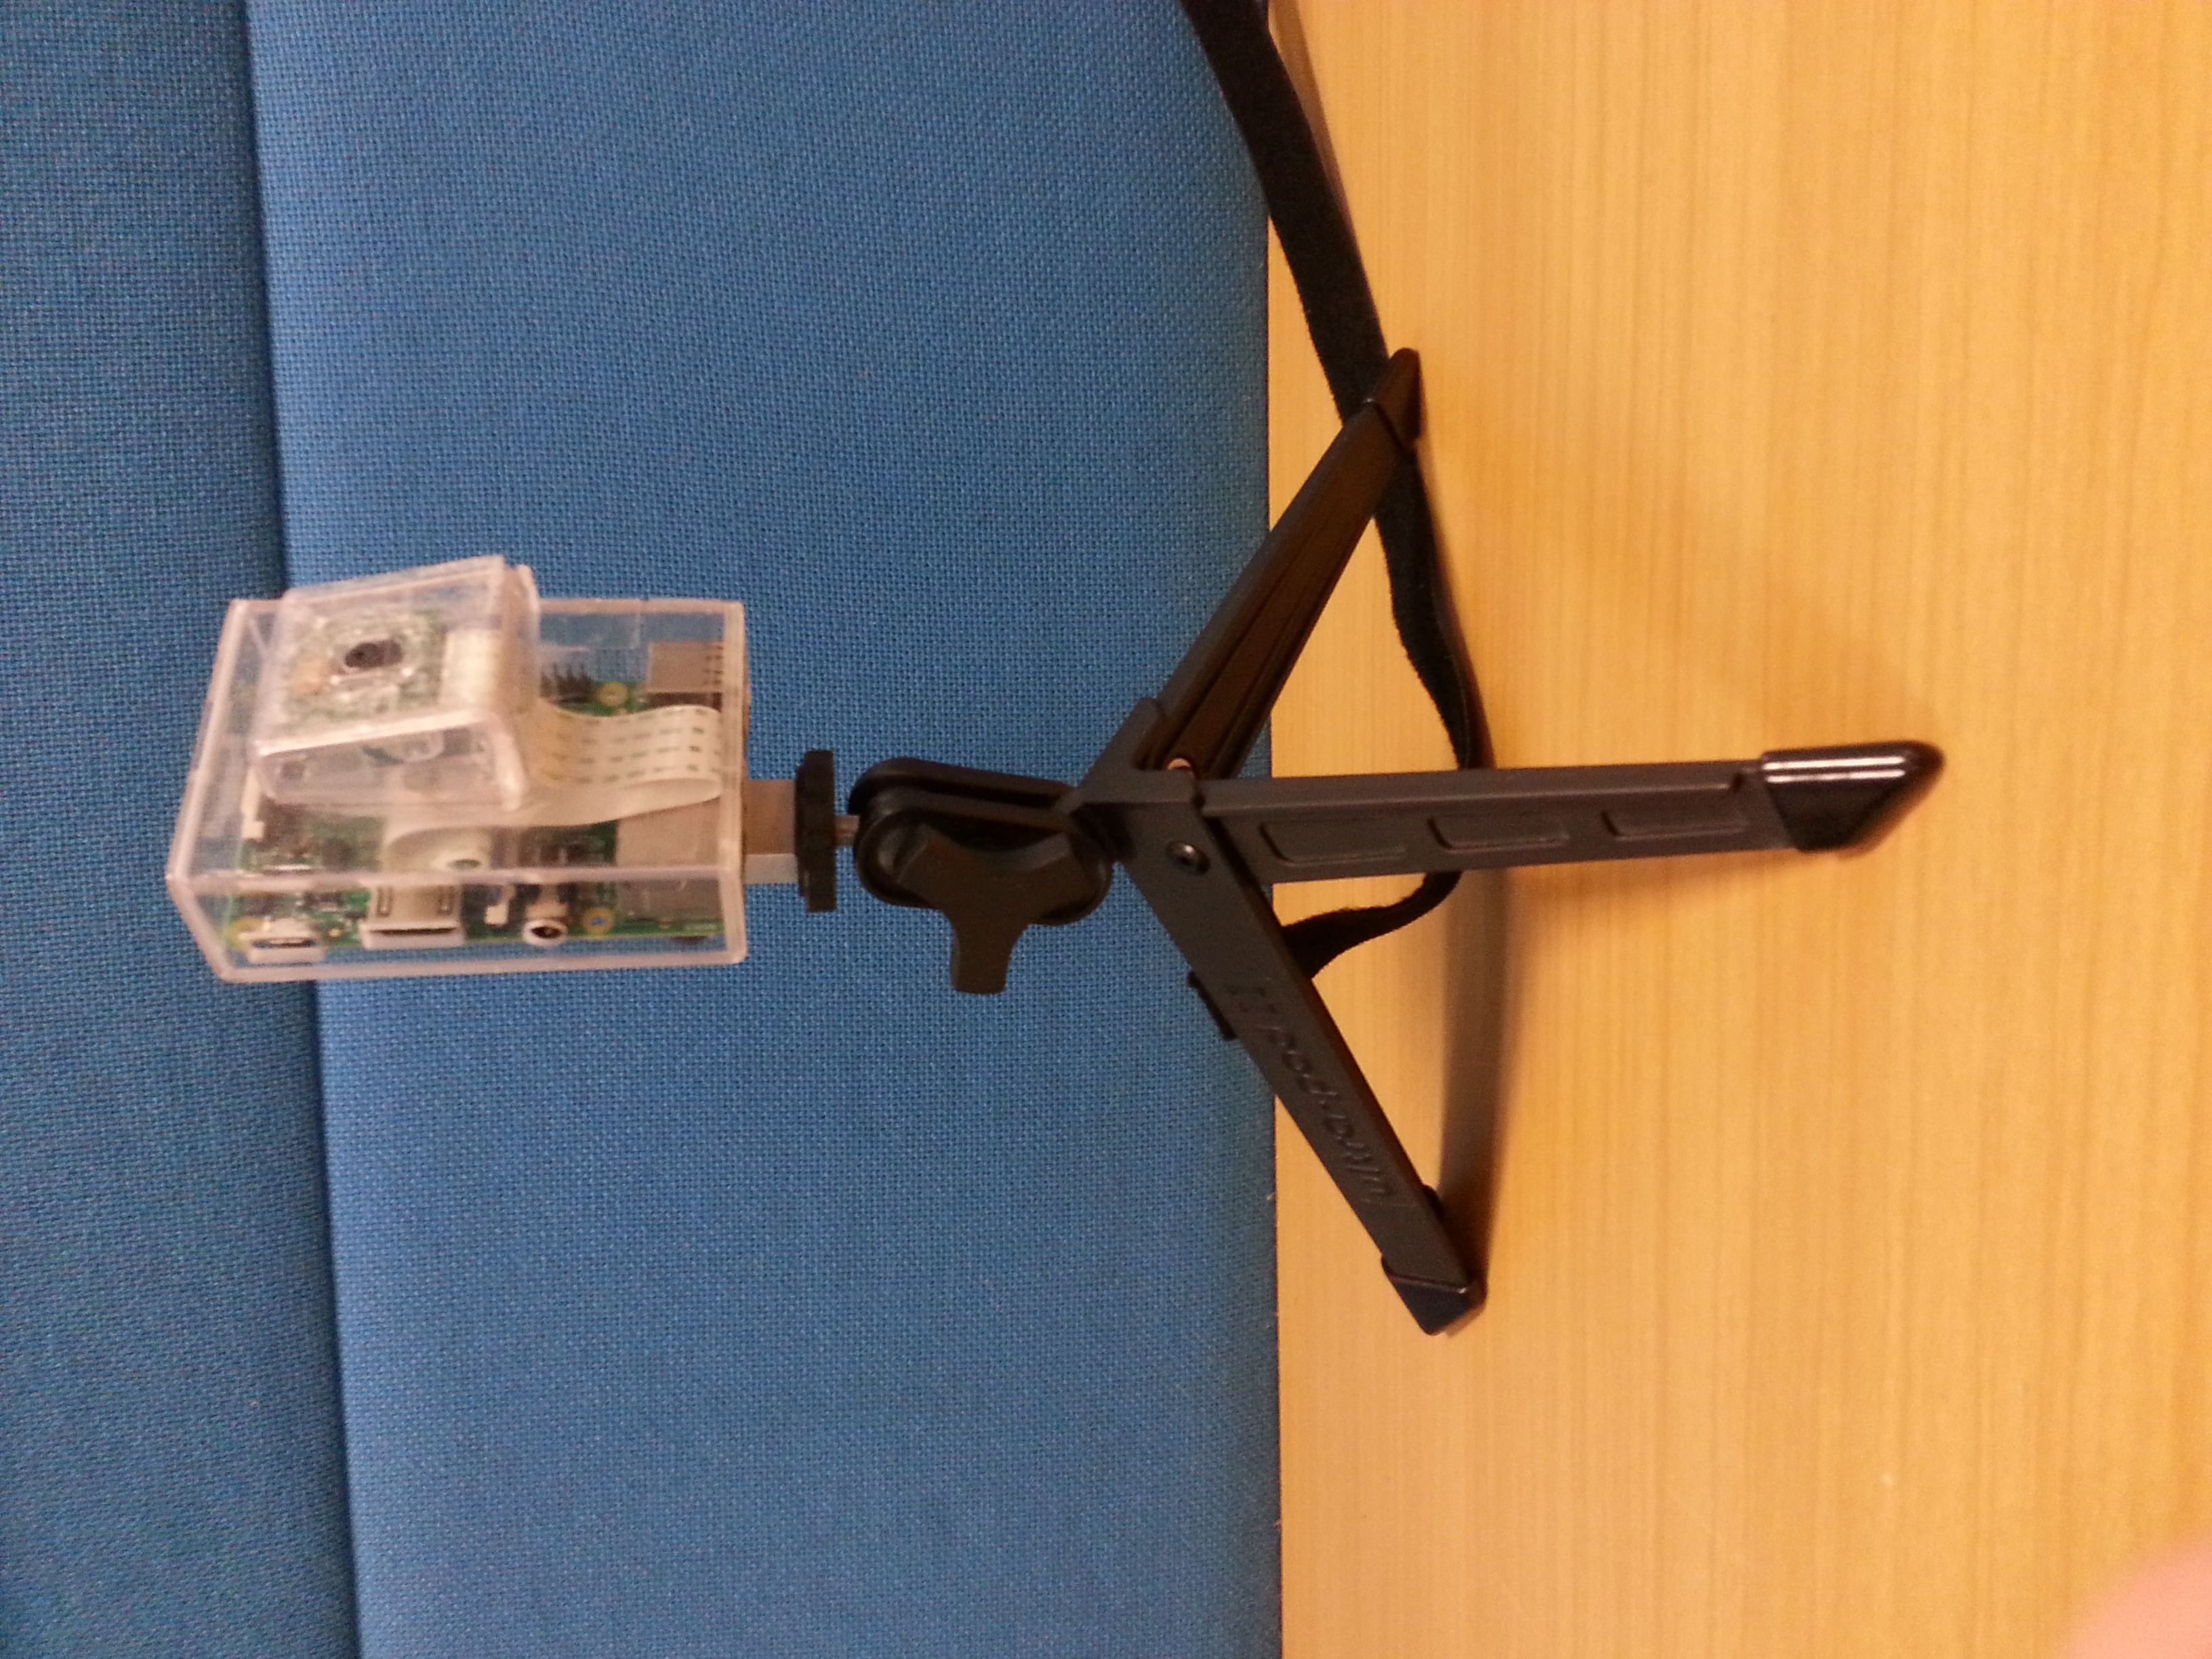
\includegraphics[height=6cm]{./pictures/raspberry}
	\label{fig:raspberryC}}
	\end{subfigure}
	\caption[Sistema di acquisizione basato su Raspberry Pi]{Il Raspberry Pi (a) e il sistema di acquisizione basato su di esso (b)}
\end{figure}
Per interfacciarci con il dispositivo abbiamo creato una \textit{connessione SSH}, tramite USB, con uno smartphone: in questo modo abbiamo potuto lanciare i comandi necessari per far partire l'acquisizione. 
Per l'acquisizione abbiamo creato uno script in \textit{Python}, utilizzando la libreria \textit{picamera} \cite{picamera} per interfacciarci con il modulo camera.\\
Abbiamo acquisito, infine, un terzo dataset utilizzando il sito \textit{ilMeteo.it}.
Questo portale di previsioni del tempo fornisce l'accesso ai frame acquisiti dalle webcam presenti in varie citt\`a e in varie localit\`a turistiche.
A ciascuna webcam \`e associato un unico URL, in cui \`e presente un'immagine in formato \textit{jpeg} rappresentante il frame corrente acquisito dalla camera.
Queste webcam, in genere, acquisiscono un frame ogni minuto, e ci\`o ha permesso di utilizzarle come caso d'uso reale.\\
Attraverso uno script in Python e il tool \textit{curl} \cite{curl}, che permette il trasferimento di dati da indirizzi URL, abbiamo creato delle sequenze di frame che coprono un arco di $24$ ore ciascuna, con frame acquisiti ogni minuto.
In questo modo abbiamo potuto valutare il comportamento degli indicatori in condizioni di framerate basso e su lunghi periodi.
\subsection{Eventi di tampering}
\label{tamperingSint}
Per testare i nostri algoritmi, abbiamo dovuto creare degli eventi in cui venisse compromessa l'acquisizione corretta della scena ripresa.
Nel caso del dataset acquisito con il Raspberry Pi abbiamo potuto introdurre degli eventi di tampering \textit{reali}, ad esempio spostando la camera durante la ripresa, oppure buttando dell'acqua o spruzzando del deodorante spray sull'obiettivo della camera, in modo da creare la sfocatura.\\
Nel caso dei frame presi dalle webcam su internet abbiamo dovuto creare degli eventi di tampering in maniera \textit{sintetica}.
La sfocatura \`e stata introdotta utilizzando delle convoluzioni con filtri \textit{gaussiani} di varie dimensioni,
\begin{equation}
\label{eq:blurArtificiale}
z_t(x) = \left\{ \begin{array}{ccl}
z_t(x) & \mbox{per} & t=1,\dots,T^* -1 \\
(z_t \circledast f)(x) & \mbox{per} & t > T^* 
\end{array}\right. , \forall x \in \mathcal{X},
\end{equation}
dove $f$ \`e ottenuto tramite un campionamento della \textit{funzione gaussiana} $h$, con media $0$ e deviazione standard $\sigma$, descritta in \eqref{eq:gaussian}.
Per creare sfocature di intensit\`a differente abbiamo utilizzato filtri gaussiani di dimensioni varie e deviazioni standard $\sigma$ differenti.\\
Lo spostamento della camera, invece, \`e stato simulato concatenando sequenze di frame differenti.
\subsection{Definizione dei ground truth}
Per valutare le prestazioni del nostro metodo, abbiamo dovuto definire un \textit{ground truth} (GT) per ciascuna sequenza video, in modo da poter disporre di alcune metriche per poter confrontare i risultati ottenuti.\\
Dato che il nostro algoritmo identifica gli istanti in cui un evento di tampering inizia, nel GT di ciascuna sequenza sar\`a presente, quindi, il numero del frame in cui questo evento inizia effettivamente. 
In particolare avremo un'indicazione del frame in cui avviene una sfocatura (se presente) e un'indicazione del frame in cui avviene lo spostamento della camera (se presente).
Ricordiamo, inoltre, che nella nostra analisi stiamo considerando che il passaggio da una situazione prima di tampering a una con tampering come un evento \textit{istantaneo}. 
\section{Figure di merito}
\label{figureDiMerito}
Grazie all'informazione presente nel GT siamo in grado, una volta che viene lanciato l'algoritmo di tampering detection, di definire quando il risultato \`e corretto e quando no.
Combinando assieme i risultati ottenuti possiamo ricavare delle cifre di riferimento che ci permettano di valutare le prestazioni del nostro algoritmo.
\subsection{Creazione delle ROC curve per il monitoraggio one-shot}
\label{metricheOneShot}
Le ROC curve forniscono un metodo grafico per la valutazione della qualit\`a delle tecniche di monitoraggio one-shot che vogliamo confrontare.\\
Per la loro costruzione, come prima cosa, \`e necessario valutare alcuni indicatori.
Come abbiamo visto nel Paragrafo \ref{monitoraggio}, dato un generico descrittore $\xi(t)$ e il suo detrending $\frac{\partial \xi}{\partial t}(t)$, il monitoraggio one-shot che viene fatto sul detrending utilizza due soglie $\Gamma_{min}^\xi$ e $\Gamma_{max}^\xi$, definite come:
\begin{equation}
	\label{eq:soglieGeneriche}
	\begin{array}{lcl}
	\Gamma_{min}^\xi & = & \widehat{\mu}_\xi -\gamma \widehat{\sigma}_\xi\\
	\Gamma_{max}^\xi & = & \widehat{\mu}_\xi + \gamma \widehat{\sigma}_\xi
	\end{array},
\end{equation}
dove $\widehat{\mu}_\xi$ indica il valore medio delle osservazioni del training set
\begin{equation}
\widehat{\mu}_\xi = \frac{\sum_{\tau = 1}^{T_{o}} \frac{\partial \xi}{\partial t}(\tau)}{T_{o}}, \nonumber
\end{equation}
$\widehat{\sigma}_\xi$ indica la deviazione standard delle osservazioni del training set
\begin{equation}
\widehat{\sigma}_\xi  = \sqrt{\frac{1}{T_{o}-1}\sum_{\tau=1}^{T_{o}}\left(\frac{\partial \xi}{\partial t}(\tau) - \widehat{\mu}_\xi(\tau)\right)^2} \nonumber
\end{equation}
e $\gamma>1$ \`e un parametro moltiplicativo.\\
Fissato un valore di $\gamma$, una volta che abbiamo lanciato il monitoraggio per un consistente numero di sequenze di frame con eventi di tampering, quello che andiamo a controllare \`e:
\begin{itemize}
	\item il numero totale di \textbf{true positive} (TP), ovvero le identificazioni avvenute correttamente;
	\item il numero totale di \textbf{true negative} (TN), ovvero il numero di frame che, giustamente, non vengono identificati dall'algoritmo;
	\item il numero totale di \textbf{false positive} (FP), ovvero il numero di frame che vengono identificati dall'algoritmo ma che non corrispondono a un evento di inizio di tampering;
	\item il numero totale di \textbf{false negative} (FN), ovvero il numero di eventi di inizio tampering che non vengono individuati dall'algoritmo.
\end{itemize}
Queste cifre di merito vengono calcolate per diversi valori del parametro $\gamma$, utilizzato per la definizione delle soglie in \eqref{eq:soglieGeneriche}.
Una volta trovati tutti i valori possiamo realizzare un grafico, dove:
\begin{itemize}
	\item Sull'asse delle ascisse mettiamo il valore \textit{1-SPECIFICITY} al variare di $\gamma$:
	\[1-\text{SPECIFICITY}_\gamma = 1-\frac{\text{TN}_\gamma}{\text{TN}_\gamma+\text{FP}_\gamma}=\frac{\text{FP}_\gamma}{\text{TN}_\gamma+\text{FP}_\gamma}\]
	\item Sulle ordinate mettiamo il valore \textit{RECALL} al variare di $\gamma$:
	\[\text{RECALL}_\gamma=\frac{\text{TP}_\gamma}{\text{TP}_\gamma+\text{FN}_\gamma} \]
\end{itemize}
Il risultato finale \`e una curva che passa per i punti $(0,0)$ e $(1,1)$, che corrispondono rispettivamente ai casi in cui i valori di soglia sono troppo alti (e quindi non viene identificato nessun evento di tampering) o sono troppo bassi (e quindi tutti i dati vengono considerati come tampering).
L'area sottesa a ciascuna curva prende il nome di \textit{Area Under Curve} della ROC (AUC) e il suo valore fornisce un elemento di confronto fra tecniche diverse.  
Dato uno specifico tampering, quindi, possiamo scegliere la tecnica la cui ROC curve ha un valore di AUC pi\`u elevato.
Inoltre, grazie alle ROC curve, possiamo ricavare il valore ottimale del parametro $\gamma$, cercando quello per cui la curva \`e pi\`u vicina al punto $(0,1)$.
%Per lo spostamento della camera abbiamo che:
%\begin{itemize}
%	\item in generale l'approccio "a regioni" ha prestazioni migliori dell'approccio su tutta la scena
%	\item l'analisi dell'energia media della luma va meglio del frame difference
%\end{itemize}

\subsection{Metriche per il monitoraggio sequenziale}
Per valutare le prestazioni del monitoraggio sequenziale, abbiamo analizzato i valori di alcuni indicatori al variare dell'intensit\`a della sfocatura presente nelle immagini affette da tampering.
Abbiamo fatto questa valutazione solamente per gli eventi di tampering creati artificialmente; l'intensit\`a della sfocatura, in questo modo, \`e determinata univocamente dalla larghezza del filtro $f$, utilizzato in \eqref{eq:blurArtificiale} per la creazione della sfocatura, e dalla sua deviazione standard $\sigma$.\\
Se indichiamo con $T^*$ l'istante in cui avviene l'evento di sfocatura e con $\widehat{T}$ la sua stima fatta dal monitoraggio sequenziale, le figure di merito che possiamo considerare sono:
\begin{itemize}
	\item \textbf{False Positive Rate} (FPR), ovvero la percentuale di sequenze in cui viene indicato erroneamente un evento di tampering, ovvero quando $\widehat{T}<T^*$.
	\item \textbf{False Negative Rate} (FNR), ovvero la percentuale di sequenze in cui non viene identificato un evento di tampering.
	\item \textbf{Detection Delay} (DD), ovvero la latenza media ($\widehat{T} - T^*$) in caso di corretta identificazione dell'evento di tampering, che si ha nel caso in cui $\widehat{T}>T^*$.
\end{itemize}

\section{Esperimento 1: tampering sintetico}
\label{esp1}
Le prime prove sperimentali che abbiamo condotto riguardano l'utilizzo di sequenze video in cui gli eventi di tampering vengono indotti sinteticamente, utilizzando le tecniche che abbiamo descritto nel Paragrafo \ref{tamperingSint}.
Abbiamo analizzato il comportamento del nostro algoritmo per varie sequenze di frame e utilizzato le cifre di merito e i grafici introdotti nel Paragrafo \ref{figureDiMerito}.
\subsection{Creazione del tampering}
Gli esperimenti sintetici sono stati condotti sia per quanto riguarda la sfocatura che per quanto riguarda lo spostamento della camera.\\
Gli eventi di sfocatura sono stati creati utilizzando la \eqref{eq:blurArtificiale}.
In particolare abbiamo considerato tre diverse scene.
Per ciascuna scena abbiamo utilizzato $10$ diversi tipi di filtro gaussiano, variando la deviazione standard $\sigma$ tra $1$ e $10$.
Inoltre, per ciascun filtro, abbiamo creato $5$ sequenze diverse, cambiando l'istante in cui avviene l'evento di sfocatura.
In totale, quindi, le sequenze video che abbiamo considerato per la nostra valutazione sono state $150$.
La Figura \ref{fig:syntDef} mostra alcuni esempi di come operano i filtri gaussiani appena definiti.\\
\begin{figure}[tbp]
	\centering
	\begin{subfigure}[]
		{\includegraphics[width=12cm]{./pictures/sequenzeCreate/defocus1}
			\label{fig:synt2}}
	\end{subfigure}
	\begin{subfigure}[]
		{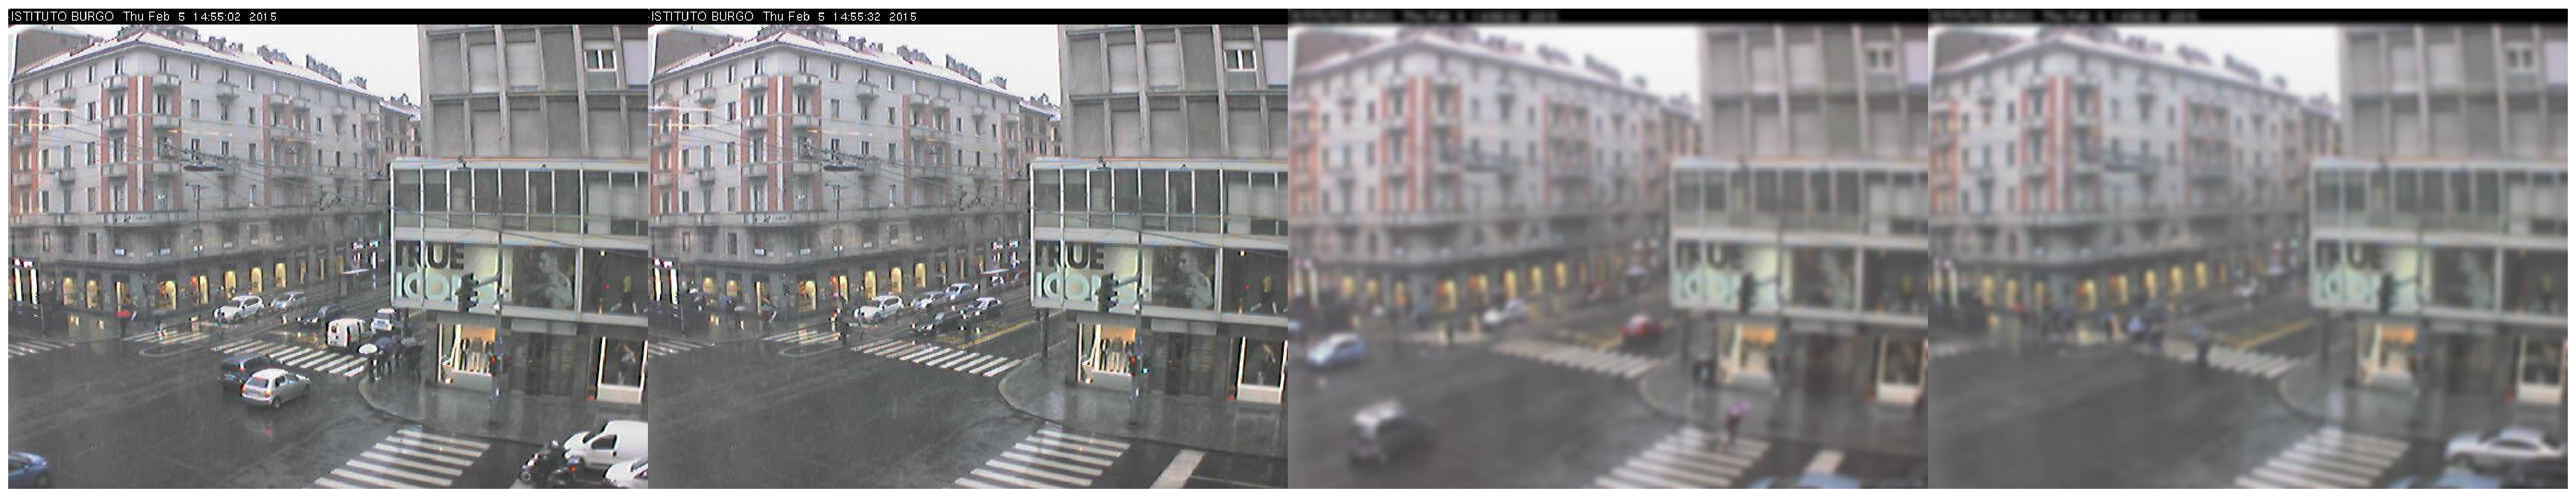
\includegraphics[width=12cm]{./pictures/sequenzeCreate/defocus3}
			\label{fig:synt3}}
	\end{subfigure}
	\begin{subfigure}[]
		{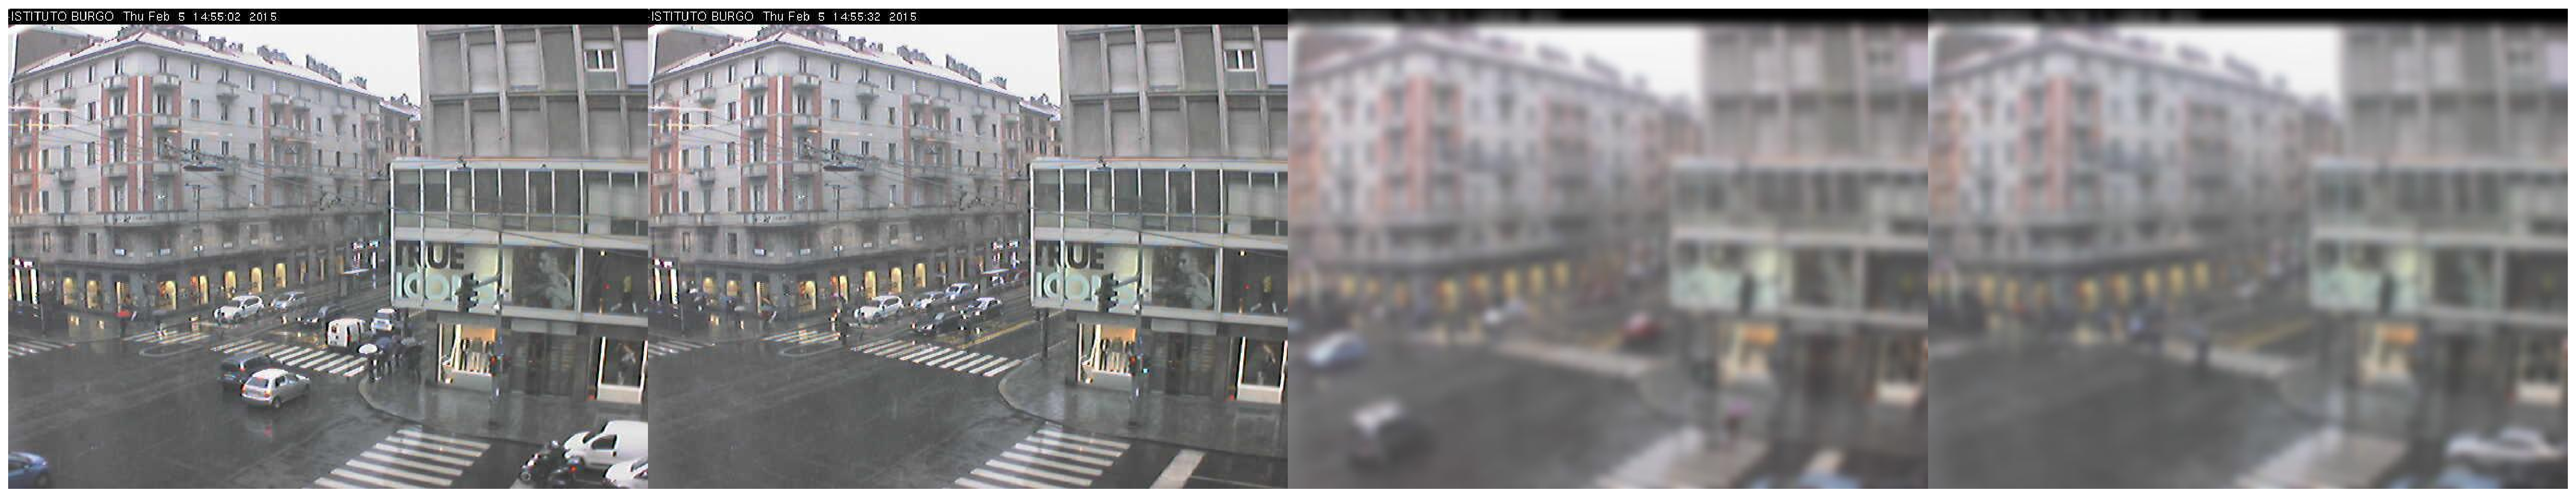
\includegraphics[width=12cm]{./pictures/sequenzeCreate/defocus5}
			\label{fig:synt4}}
	\end{subfigure}
	\begin{subfigure}[]
		{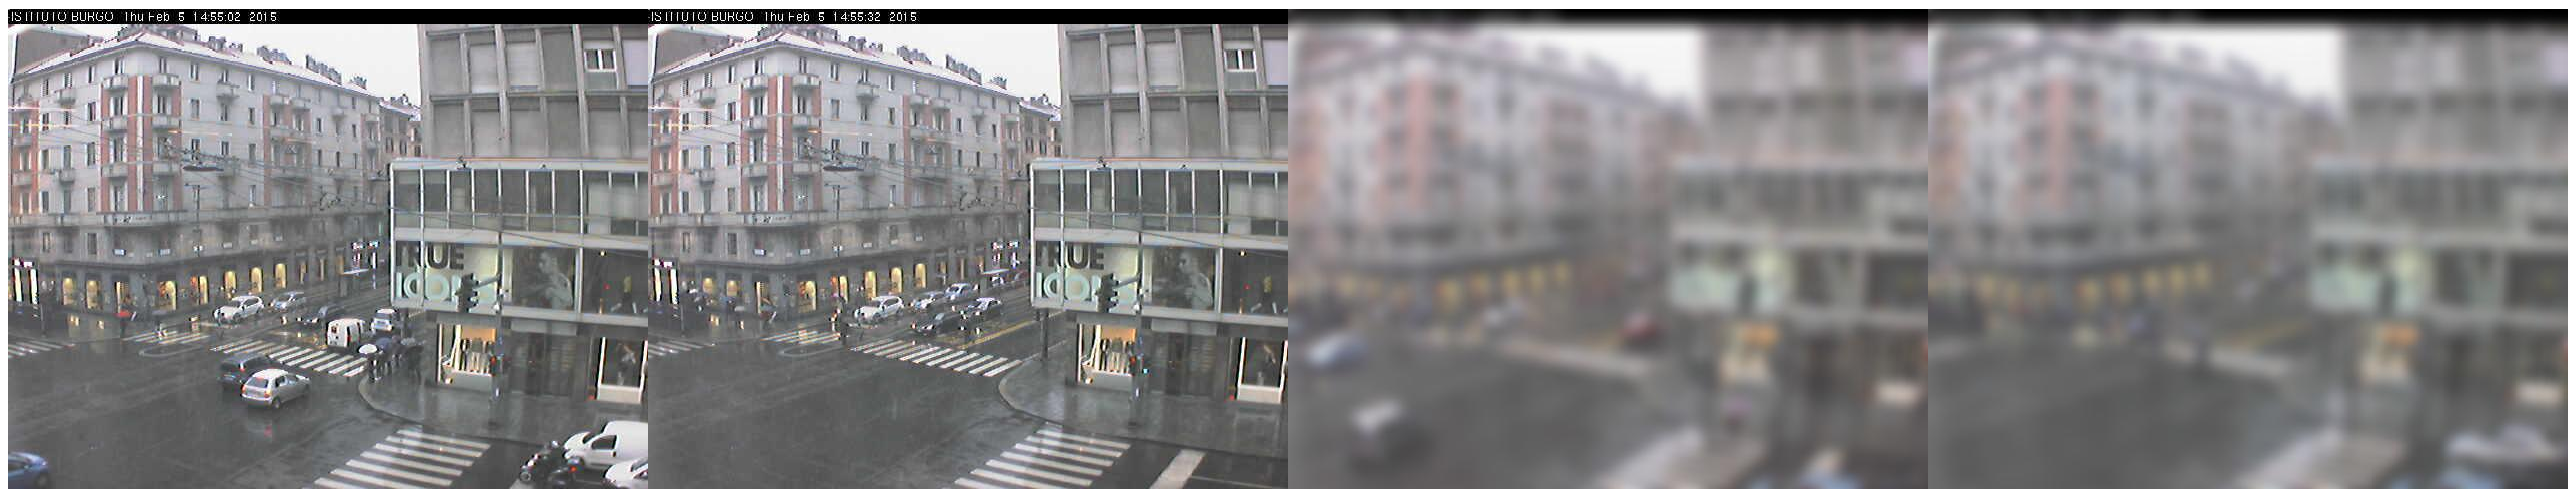
\includegraphics[width=12cm]{./pictures/sequenzeCreate/defocus7}
			\label{fig:synt5}}
	\end{subfigure}
	\begin{subfigure}[]
		{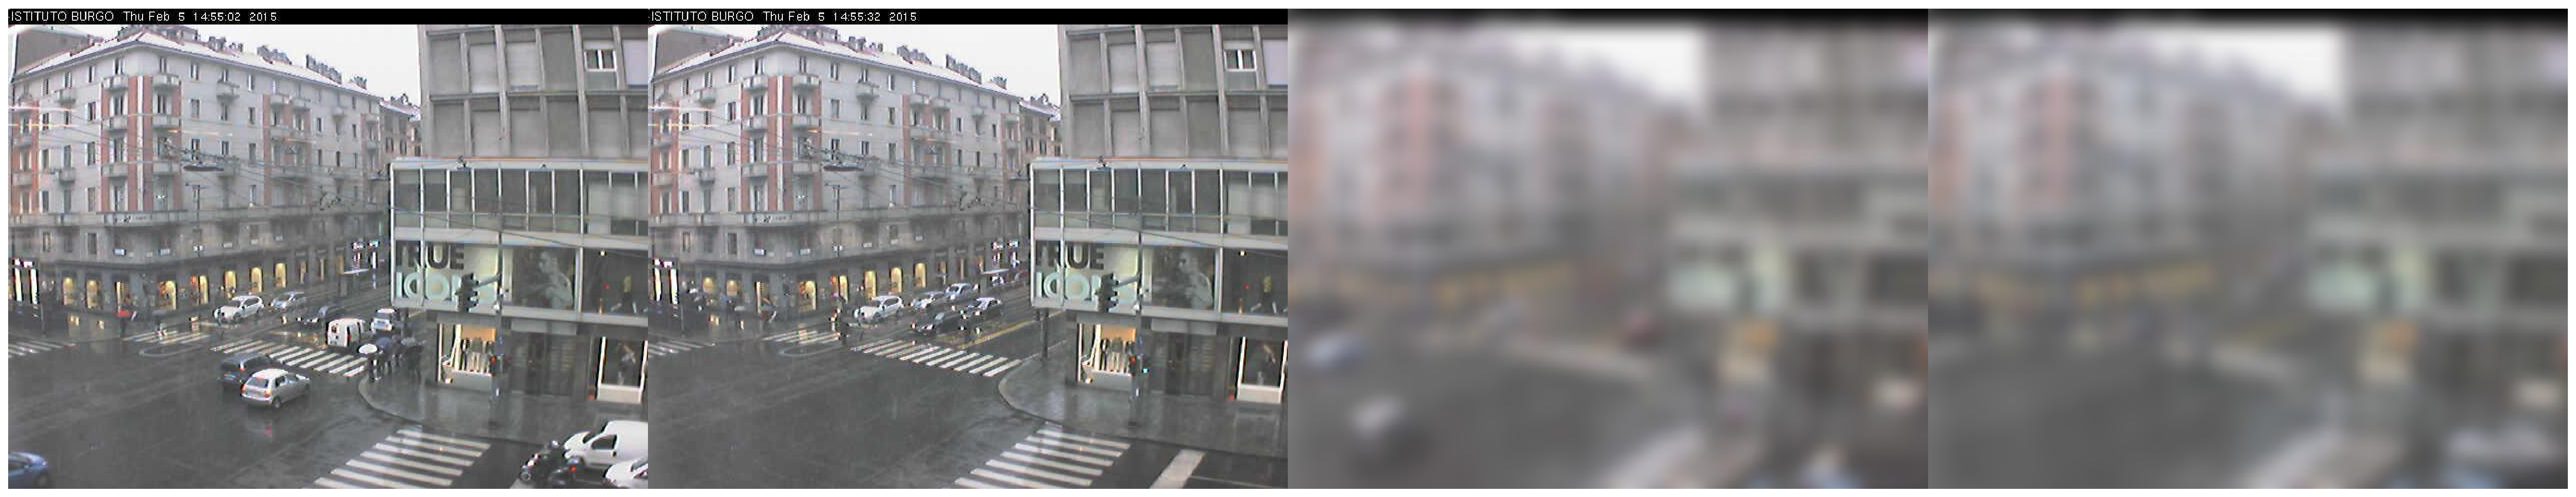
\includegraphics[width=12cm]{./pictures/sequenzeCreate/defocus10}
			\label{fig:synt6}}
	\end{subfigure}
	\caption[Esempi di sequenze con eventi di sfocature create sinteticamente]{Esempi di sequenze con eventi di sfocature create con filtri gaussiani: (a) $\sigma=1$, (b) $\sigma=3$, (c) $\sigma=5$, (d) $\sigma=7$, (e) $\sigma=10$. }
	\label{fig:syntDef}
\end{figure}
Per simulare l'evento di spostamento della camera, invece, abbiamo creato $100$ sequenze di frame concatenando due diversi scenari tra loro.
Per rendere la simulazione il pi\`u verosimile possibile, le sequenze video concatenate hanno dovuto rispettare alcuni vincoli:
\begin{itemize}
	\item le acquisizioni di entrambe le sequenze devono avvenire nello stesso giorno e negli stessi istanti di tempo;
	\item lo scenario ripreso dalle due sequenze deve essere simile; ad esempio, nel nostro caso, entrambe le sequenze video riprendevano strade trafficate,
	\item le due camere che eseguono l'acquisizione devono essere posizionate a un'altezza simile; ad esempio, nel nostro caso, le due camere erano entrambe poste al primo piano di un palazzo,
	\item le due camere che eseguono l'acquisizione devono essere orientate in maniera \textit{diversa} tra loro.
\end{itemize}
La Figura \ref{fig:syntDispl} mostra un esempio di sequenze concatenate tra loro per simulare l'evento di spostamento della camera.
\begin{figure}[tb]
	\centering
	\includegraphics[width=13cm]{pictures/sequenzeCreate/displacement}
	\caption{Esempio di sequenza con un evento di spostamento della camera creato sinteticamente}
	\label{fig:syntDispl}
\end{figure}

\subsection{Risultati}
\begin{figure}[tb]
	\centering
	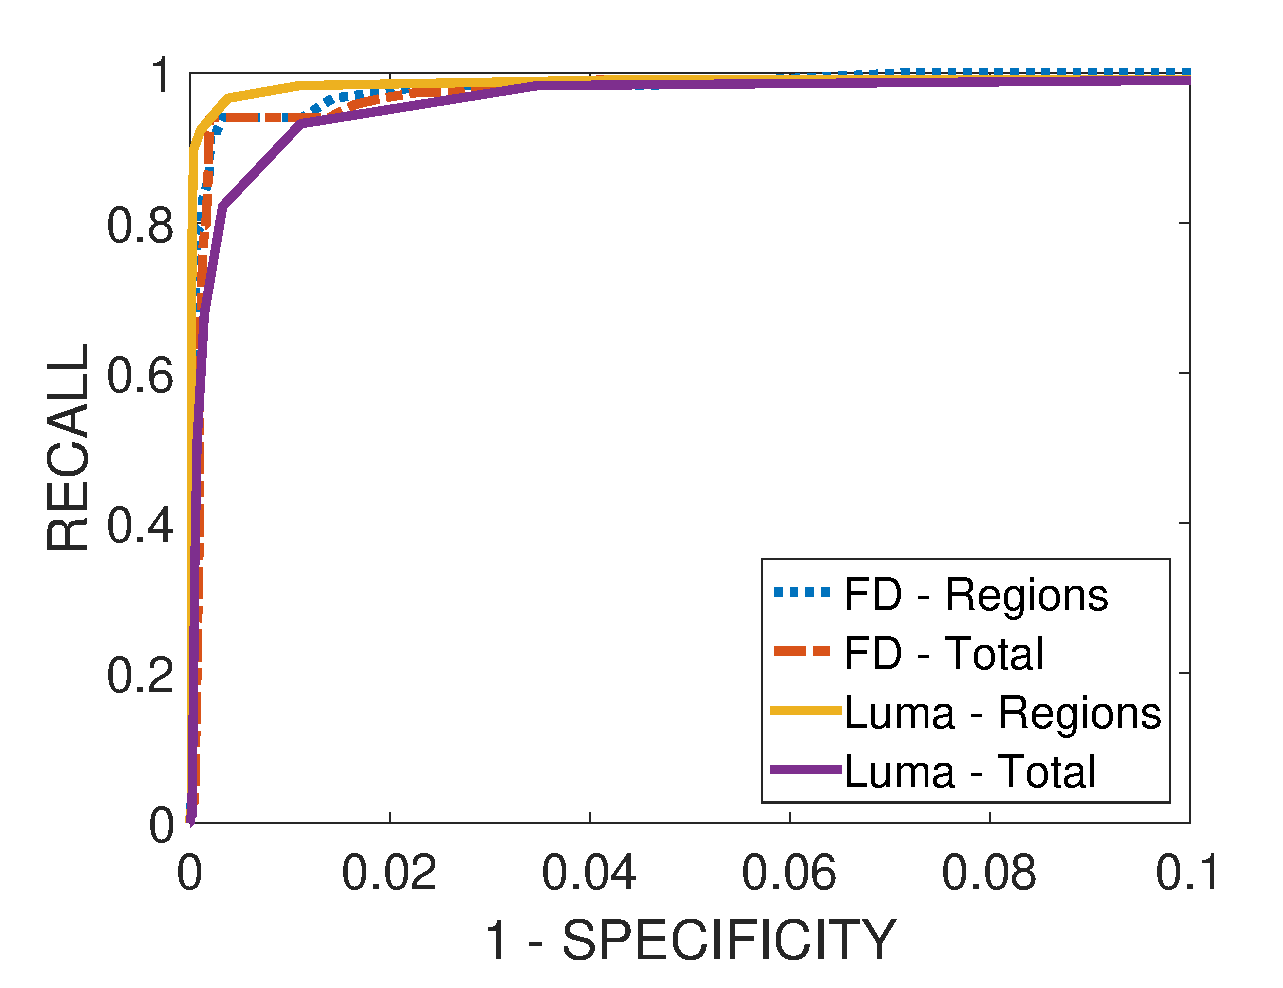
\includegraphics[width=13cm]{diagrammi/ROC_displacement}
	\caption{Curve ROC per gli indicatori di spostamento della camera}
	\label{fig:ROC_displacement}
\end{figure}
%
%Per la sfocatura non abbiamo vantaggi ad utilizzare la segmentazione rispetto alla totalit\`a della scena.\\ 
\begin{figure}[tb]
	\centering
	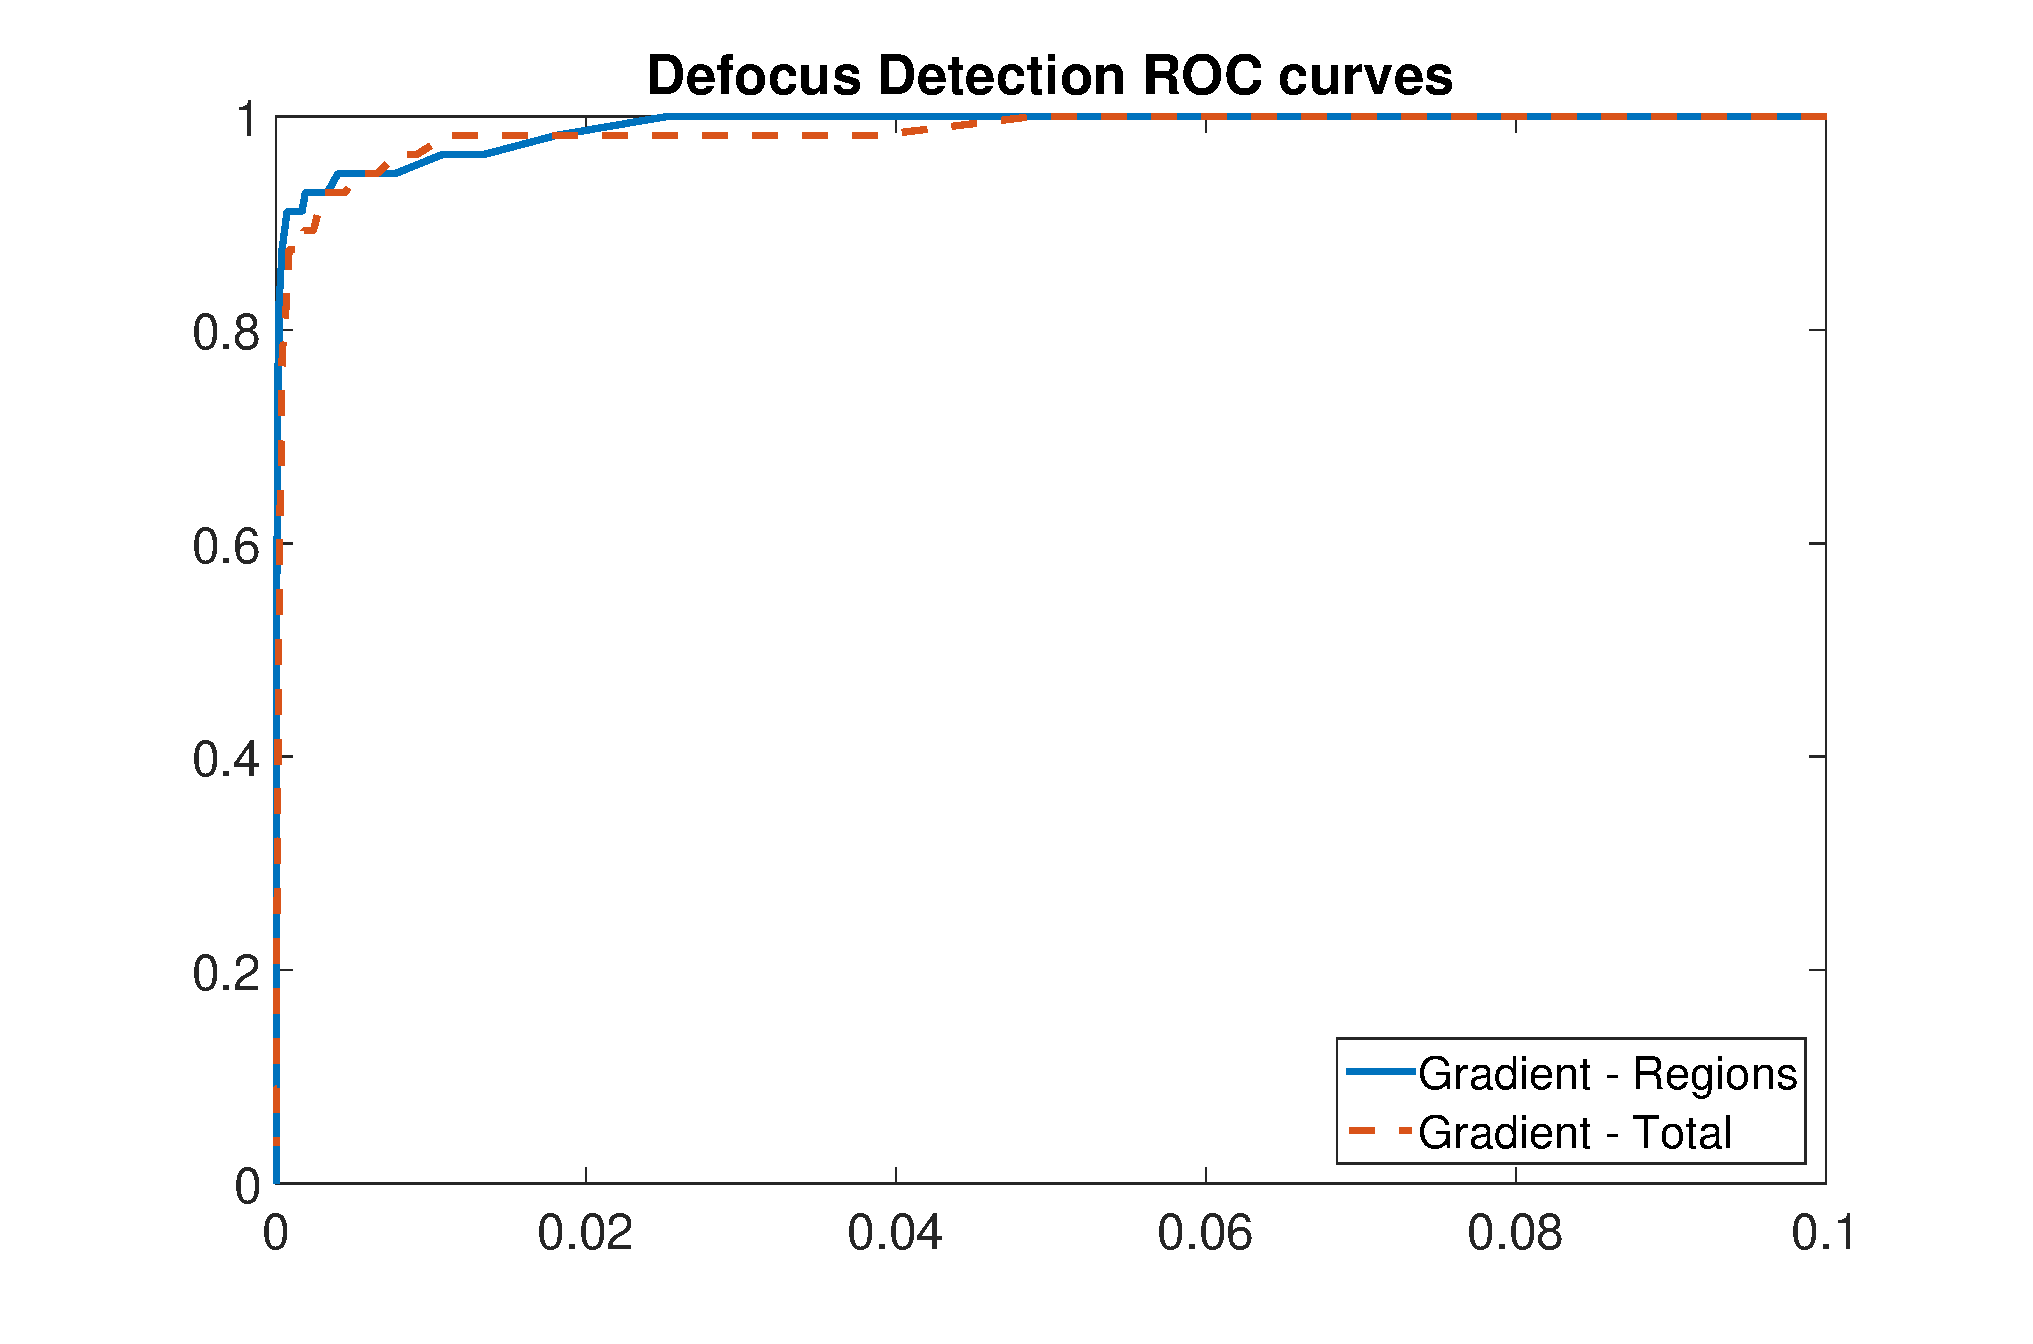
\includegraphics[width=13cm]{diagrammi/ROC_defocus}
	\caption{Curve ROC per gli indicatori di sfocatura}
	\label{fig:ROC_defocus}
\end{figure}
\begin{figure}[tb]
	\centering
	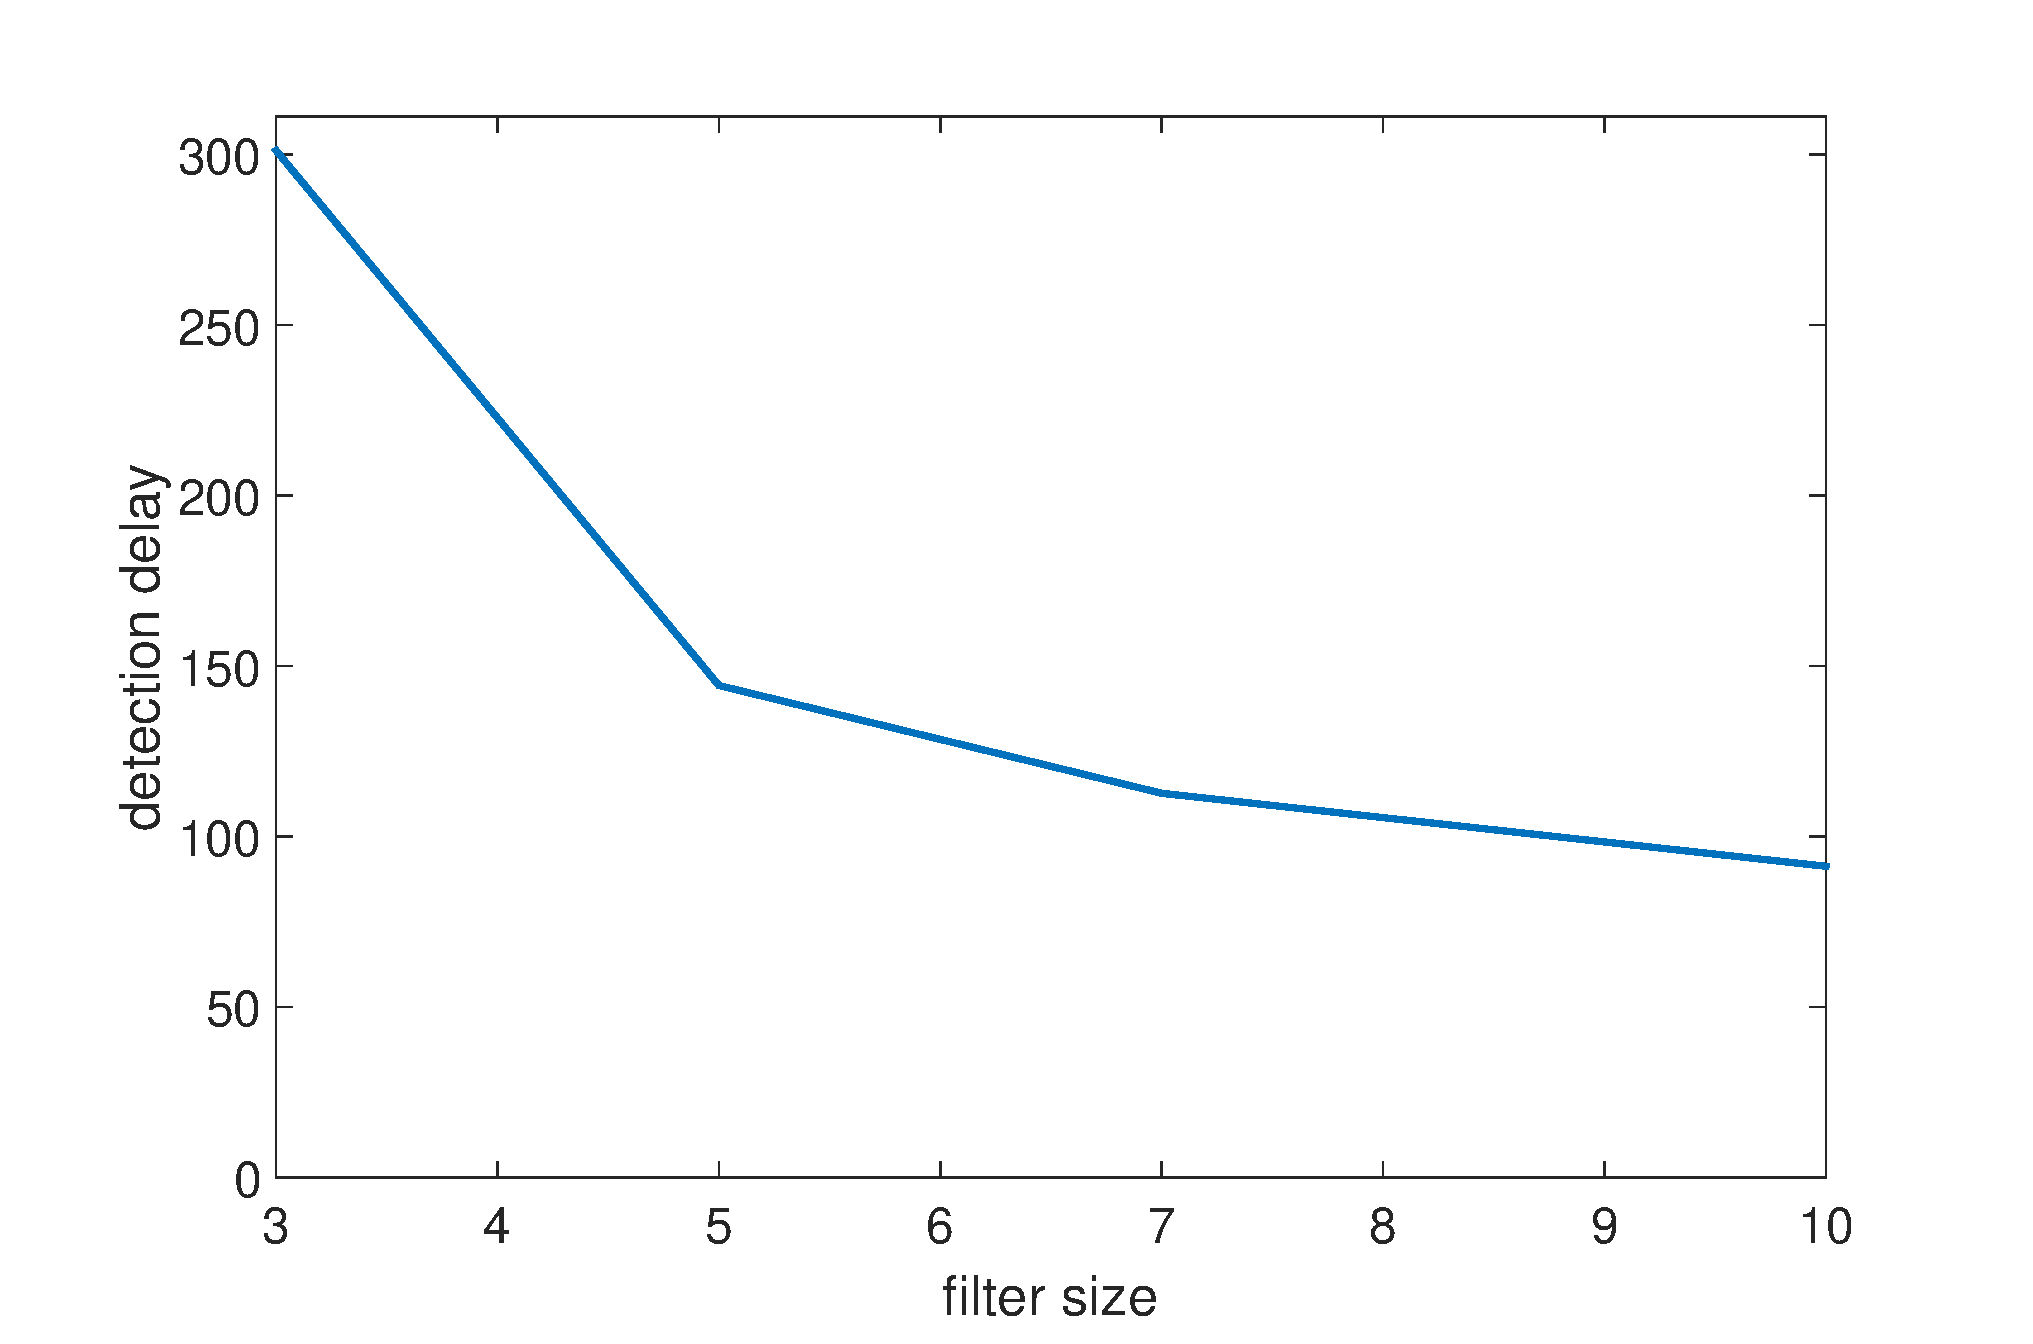
\includegraphics[width=13cm]{diagrammi/DD}
	\caption{Detection Delay per l'analisi sequenziale della varianza dell'energia del gradiente}
	\label{fig:DD}
\end{figure}
\begin{figure}[tb]
	\centering
	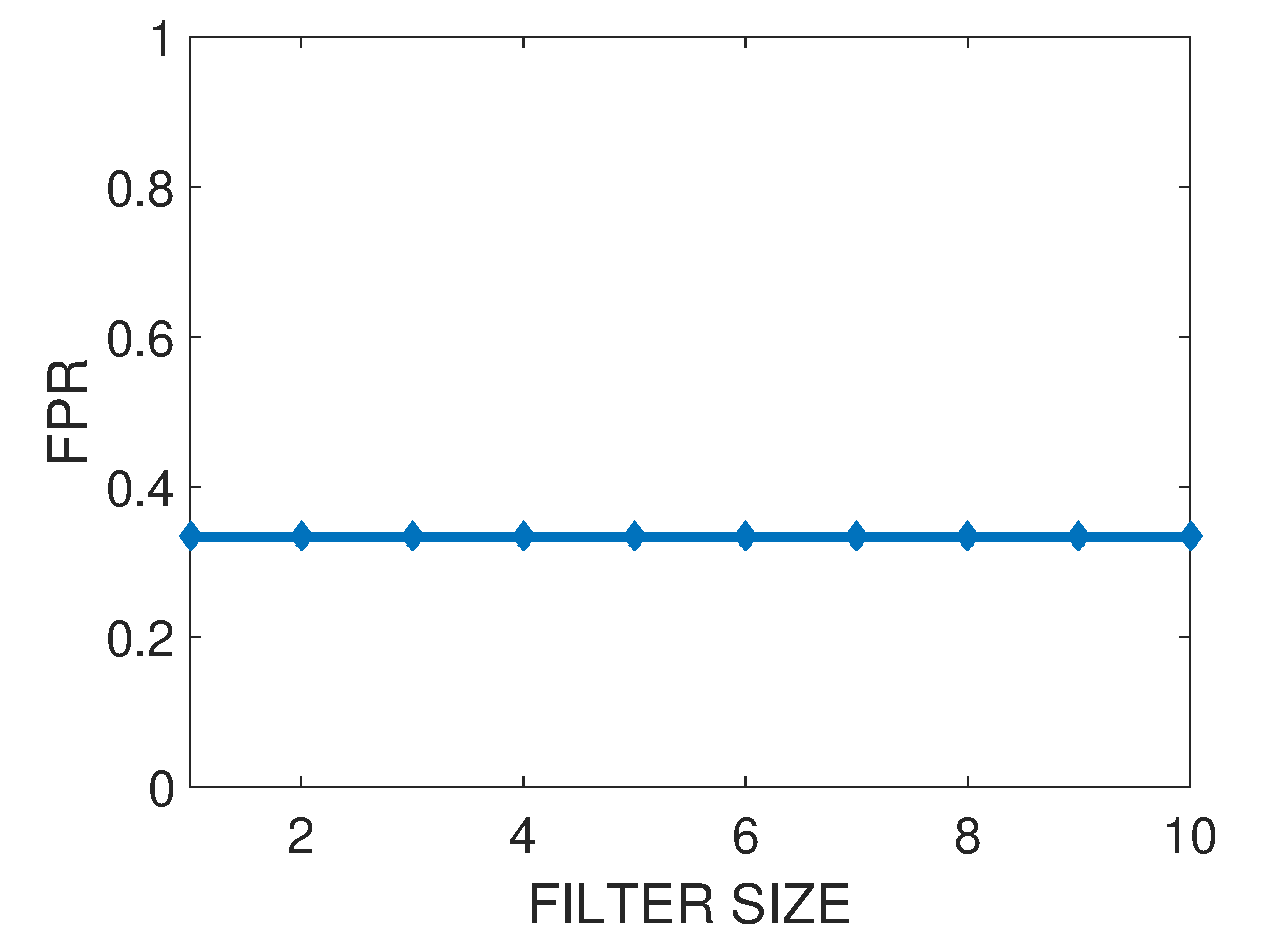
\includegraphics[width=13cm]{diagrammi/FPR}
	\caption{False Positive Rate per l'analisi sequenziale della varianza dell'energia del gradiente}
	\label{fig:FPR}
\end{figure}
\begin{figure}[tb]
	\centering
	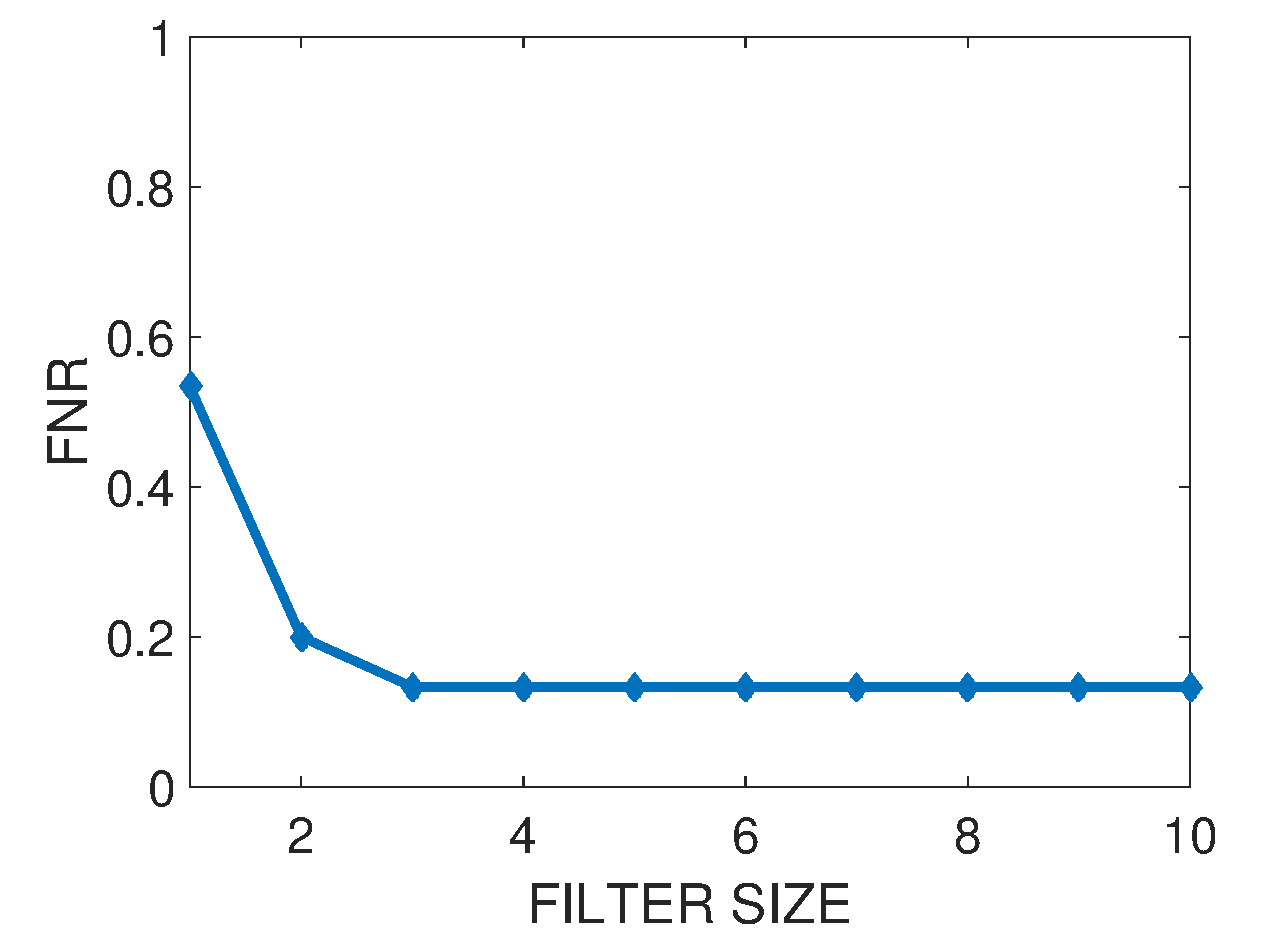
\includegraphics[width=13cm]{diagrammi/FNR}
	\caption{False Negative Rate per l'analisi sequenziale della varianza dell'energia del gradiente}
	\label{fig:FNR}
\end{figure}
\section{Esperimento 2: tampering reale}
\label{esp2}

